\documentclass{beamer}
\usepackage[utf8]{inputenc}
\usepackage[russian]{babel}
\usepackage{xcolor}
\usepackage{geometry}
\usetheme{texsx}







\begin{document}



\begin{frame}[plain]
\begin{tikzpicture}[remember picture,overlay]
\node[at=(current page.center)] {
    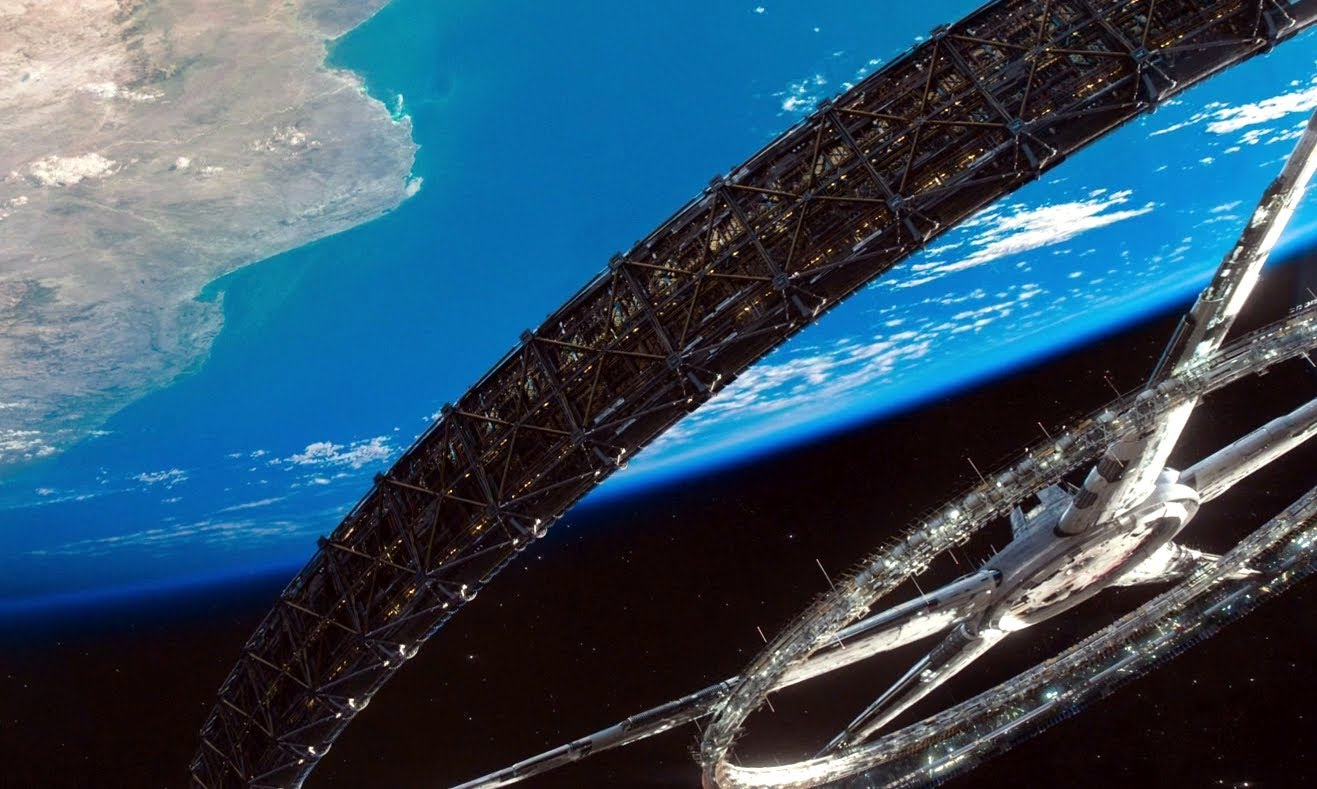
\includegraphics[width=\paperwidth, height=\paperheight, keepaspectratio]{elysium.jpg}
};
\end{tikzpicture}
 \end{frame}

\begin{frame}\frametitle{Fanera (1715)}
\begin{center}
\begin{tikzpicture}
\node[draw=accent,line width=1mm,inner sep=1] at(0,0) {\includegraphics[height=7cm]{pilewood.jpg}};
\end{tikzpicture}
\end{center}
\end{frame}

\begin{frame}\frametitle{Anaxagor}
\begin{columns}
\column{4.2cm}
\begin{center}
\begin{tikzpicture}
\node[draw=accent,line width=1mm,inner sep=1] at(0,0) {\includegraphics[width=4cm]{anaxagor.jpg}};
\end{tikzpicture}
(годы)
\end{center}
\column{6cm}
Не я потерял Афины - Афины потеряли меня
\end{columns}
\end{frame}



\end{document}